\chapter{\IfLanguageName{dutch}{Evaluatie van resultaten}{Results Evaluation}}%
\label{ch:results}

As expected the application is effectively published for all platforms available from a x86/x64-CPU based computer using one single codebase. Making builds for Apple ecosystem devices like iPhone or Mac, requires macOS with Xcode installed what was unavailable during the research but can be a subject of further works.


\section{{Development phase}}%
\label{sec:development_evaluation}

The development phase was relatively efficient, despite some problems when making build for Electron on Linux described is Cross platform builds chapter \ref{sec:desktop}.

There are some important facts to consider about Electron framework. It is based on Google Chromium browser and has relatively short support period for each release (about 6 months) and LTS versions are not available. In some cases for security reasons the application will require regular updates following Chromium and Electron calendar. If developers decide to publish the product on Microsoft Store, it will be necessary to comply with requirement that  browser-based apps have to be within two major versions of the latest release of the browser engine\autocite{MSstoreElectron}.

\begin{table}[H]
    \centering
    \begin{tabular}{lcccccc}
        \toprule
        Release & Status & Released & End of life & Chromium & Node.js\\
        \midrule
        v33.x.y  &  End-of-Life  &  15-10-2024  &  29-04-2025  &  130  &  20.18   \\
        v34.x.y  &  Active  &  14-01-2025  &  24-06-2025  &  132  &  20.18   \\
        v35.x.y  &  Active  &  4-03-2025  &  2-09-2025  &  134  &  22.14   \\
        v36.x.y  &  Current  &  29-04-2025  &  28-10-2025  &  136  &  22.14   \\
        v37.x.y  &  Prerelease  &  24-06-2025  &  13-01-2026  &  138  &  TBD   \\ 
        \bottomrule
\end{tabular}
\caption[Electron version history]{\label{tab:electronhistory}Electron version history and support dates \autocite{ElectronReleases}.
}
\end{table}


\section{{UI uniformity and appearance, user experience}}%
\label{sec:appseveluation}
Mediko on Electron Desktop delivers similar user experience as in a web browser, on mobile device the application works like a native Android app.

Despite application look almost identically on all platforms there was an issue discoverd. On Google Chrome browser, the account link on the drawer panel during mouse move is displayed in the middle of the page height and a scroll bar appears at the bottom of the drawer. There are some differences between web-browsers how they render html pages with CSS, an explanation is provided by a Medium.com blogger in article 'Why Your CSS Looks Different on Every Browser?' \autocite{MediumCSS}. The issue will be described as a bug in Azure DevOps project.

\begin{figure}[H]
    \centering
    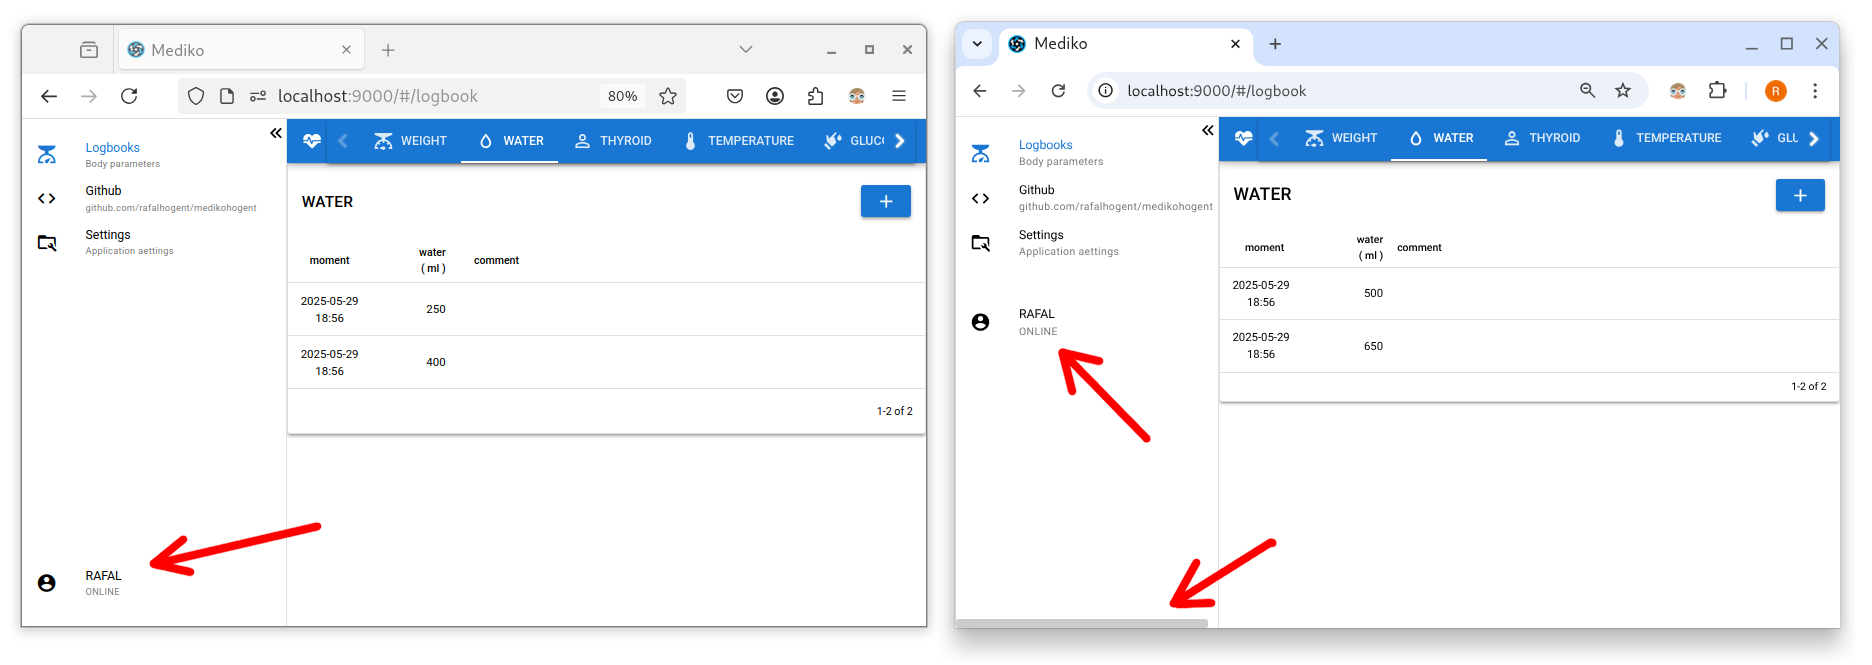
\includegraphics[width=1\textwidth]{chromeissue.png}
    \caption[CSS rendering issue]{\label{fig:chromeissue} Different positions of the Account link. FIrefox (left), Chrome (right). Scrollbar visible at the bottom of Chrome's sidebar.}
\end{figure}

\section{{Size, stability, performance}}%
\label{sec:sizeapps}
For the purpose of the proof-of-concept application the performance is completely sufficient. On all platforms program starts immediately. There were no stability issues recorded. What is worth noting, the size of cordova android .apk build is only 3.5MB, compared to Native React about 70 MB for a similar functionality application.

\begin{table}[H]
    \centering
    \begin{tabular}{lcccccc}
        \toprule
        framework & platform & size \\
        \midrule
        SPA  &  Web  &  2.6MB   \\
        Electron  &  Linux x64  &  335MB   \\
        Electron  &  Windows x64  &  329MB   \\
        Cordova  &  Android  &  3.5MB   \\
        ReactNative*  &  Android  &  ~70MB   \\

 
        \bottomrule
\end{tabular}
\caption[Builds size comparison]{\label{tab:builds_size}Builds size comparison, *data for ReactNative build of a similar application developed by the author.
}
\end{table}

